\documentclass[11pt,openany,oneside]{book}
\usepackage[a4paper,top=25mm,bottom=23mm,left=25mm,right=22mm,headheight=24pt]{geometry}
\usepackage{fontspec}
\setmainfont{DejaVu Serif}
\setsansfont{DejaVu Sans}
\usepackage{amssymb,xcolor,graphicx,array,booktabs,longtable,tabularx,colortbl,enumitem,tikz,tcolorbox,fancyhdr,titlesec,tocloft,hyperref,eso-pic,microtype,listings}
\usetikzlibrary{arrows.meta,positioning,shapes.geometric,calc}
\definecolor{Navy}{HTML}{17365D}
\definecolor{Teal}{HTML}{007F86}
\definecolor{Pale}{HTML}{EAF6F7}
\definecolor{Gold}{HTML}{E3A72F}
\definecolor{Ink}{HTML}{293746}
\definecolor{LightGold}{HTML}{FFF5DD}
\definecolor{SoftGray}{HTML}{F4F6F9}
\definecolor{Coral}{HTML}{D95D50}
\definecolor{Rose}{HTML}{FCE8E6}
\definecolor{Violet}{HTML}{7656A6}
\definecolor{Sky}{HTML}{DCEEFF}
\hypersetup{colorlinks=true,linkcolor=Teal,urlcolor=Teal,pdftitle={Junior Software Developer -- Grade XI},pdfauthor={Vocational Education Textbook}}
\setlist[itemize]{leftmargin=1.5em,itemsep=1.5pt,topsep=2pt,parsep=0pt}
\setlist[enumerate]{leftmargin=1.7em,itemsep=2pt,topsep=2pt,parsep=0pt}
\setlength{\parindent}{0pt}\setlength{\parskip}{3pt}\setlength{\emergencystretch}{3em}
\lstdefinelanguage{Python}{sensitive=true,morecomment=[l]{\#},morestring=[b]',morestring=[b]",morekeywords={and,as,assert,break,class,continue,def,del,elif,else,except,False,finally,for,from,global,if,import,in,is,lambda,None,not,or,pass,raise,return,True,try,while,with,yield,print,input,range,len,type,int,float,str,list,dict,tuple,set}}
\lstdefinelanguage{Pseudo}{morekeywords={START,STOP,INPUT,OUTPUT,IF,THEN,ELSE,ENDIF,WHILE,DO,ENDWHILE,FOR,ENDFOR},sensitive=false}
\lstdefinestyle{webcode}{basicstyle=\ttfamily\small,keywordstyle=\color{Navy}\bfseries,commentstyle=\color{Teal},stringstyle=\color{Violet},numbers=left,numberstyle=\tiny\color{Ink!65},stepnumber=1,numbersep=8pt,showstringspaces=false,breaklines=true,frame=single,rulecolor=\color{Teal!55},backgroundcolor=\color{SoftGray},xleftmargin=2mm,framexleftmargin=2mm,aboveskip=5pt,belowskip=5pt}
\AddToShipoutPictureBG{\begin{tikzpicture}[remember picture,overlay]\draw[Navy!65,line width=.55pt] ([xshift=11mm,yshift=-11mm]current page.north west) rectangle ([xshift=-11mm,yshift=11mm]current page.south east);\draw[Teal,line width=1.6pt] ([xshift=11mm,yshift=-11mm]current page.north west)--([xshift=37mm,yshift=-11mm]current page.north west);\draw[Coral,line width=1.6pt] ([xshift=-11mm,yshift=11mm]current page.south east)--([xshift=-37mm,yshift=11mm]current page.south east);\fill[Gold] ([xshift=11mm,yshift=-11mm]current page.north west) circle (1.1mm);\fill[Violet] ([xshift=-11mm,yshift=11mm]current page.south east) circle (1.1mm);\end{tikzpicture}}
\pagestyle{fancy}\fancyhf{}
\fancyhead[L]{\raisebox{-3.5mm}[0pt][0pt]{\small\bfseries\sffamily\color{Teal} JUNIOR SOFTWARE DEVELOPER}}
\fancyhead[R]{\raisebox{-3.5mm}[0pt][0pt]{\small\sffamily\color{Navy} GRADE XI TEXTBOOK}}
\fancyfoot[C]{\tikz[baseline=(n.base)]\node[fill=Teal,draw=Gold,line width=.7pt,text=white,circle,minimum size=7mm,inner sep=1pt,font=\small\bfseries] (n) {\thepage};}
\renewcommand{\headrulewidth}{.5pt}
\renewcommand{\headrule}{\hbox to\headwidth{\color{Gold}\leaders\hrule height \headrulewidth\hfill}}
\fancypagestyle{plain}{\fancyhf{}\fancyhead[L]{\raisebox{-3.5mm}[0pt][0pt]{\small\bfseries\sffamily\color{Teal} JUNIOR SOFTWARE DEVELOPER}}\fancyhead[R]{\raisebox{-3.5mm}[0pt][0pt]{\small\sffamily\color{Navy} GRADE XI TEXTBOOK}}\fancyfoot[C]{\tikz[baseline=(n.base)]\node[fill=Teal,draw=Gold,line width=.7pt,text=white,circle,minimum size=7mm,inner sep=1pt,font=\small\bfseries] (n) {\thepage};}\renewcommand{\headrulewidth}{.5pt}\renewcommand{\headrule}{\hbox to\headwidth{\color{Gold}\leaders\hrule height \headrulewidth\hfill}}\renewcommand{\footrulewidth}{0pt}}
\titleformat{\chapter}[display]{\normalfont\sffamily\bfseries\color{Navy}}{\filleft\Large\color{Coral}\chaptername\ \thechapter}{.6ex}{\color{Teal}\LARGE\raggedright}[\vspace{.5ex}\color{Gold}\rule{\textwidth}{.8pt}]
\titlespacing*{\chapter}{0pt}{-8mm}{.5ex}
\titleformat{\section}{\Large\sffamily\bfseries\color{Teal}}{\color{Coral}\thesection}{.7em}{}
\titleformat{\subsection}{\large\sffamily\bfseries\color{Violet}}{\thesubsection}{.7em}{}
\titlespacing*{\section}{0pt}{1.2ex plus .2ex minus .2ex}{.35ex}
\titlespacing*{\subsection}{0pt}{1ex plus .2ex minus .2ex}{.3ex}
\newcommand{\keyterm}[1]{\textbf{\color{Navy}#1}}
\newcommand{\photo}[3]{\begin{center}\begin{tcolorbox}[colback=white,colframe=Teal!70,boxrule=.8pt,arc=1mm,left=2mm,right=2mm,top=2mm,bottom=2mm,width=.88\textwidth]\centering\IfFileExists{images/#1}{\includegraphics[width=.92\linewidth,height=46mm,keepaspectratio]{images/#1}}{\vspace{8mm}\textbf{#2}\par\small Visual example for this topic\vspace{8mm}}\end{tcolorbox}\end{center}{\small\textit{#3}}}
\newcommand{\reviewtitle}{\par\noindent\textbf{\color{Navy}Review Questions}\par}
\begin{document}
\begin{titlepage}\thispagestyle{empty}
\begin{tikzpicture}[remember picture,overlay]
\fill[Navy] (current page.north west) rectangle ([yshift=-11.4cm]current page.north east);
\fill[Teal] ([yshift=-11.4cm]current page.north west) rectangle ([yshift=-11.68cm]current page.north east);
\fill[Coral] ([yshift=-11.68cm]current page.north west) rectangle ([yshift=-11.82cm]current page.north east);
\draw[Gold,line width=2pt] ([xshift=22mm,yshift=-20mm]current page.north west)--([xshift=-22mm,yshift=-20mm]current page.north east);
\draw[Gold,line width=1pt] ([xshift=22mm,yshift=-103mm]current page.north west)--([xshift=-22mm,yshift=-103mm]current page.north east);
\end{tikzpicture}
\vspace*{20mm}{\color{white}\rmfamily\bfseries\fontsize{34}{40}\selectfont HANDBOOK\par}
\vspace{5mm}{\color{Gold}\rule{.72\textwidth}{1.2pt}\par}
\vspace{7mm}{\color{white}\sffamily\LARGE Junior Software Developer\par}
\vspace{3mm}{\color{white}\sffamily\large Grade XI -- IT-ITeS Vocational Education\par}
\vfill\begin{center}{\sffamily\Large\bfseries\color{Teal} Computer Systems \textbullet\ Networks \textbullet\ Python \textbullet\ Data Structures\par}\vspace{4mm}{\sffamily\large\color{Ink} A structured textbook for computing foundations, logical problem solving and introductory programming.}\end{center}
\vfill\begin{center}{\small Prepared as a learning-focused companion based on the supplied Junior Software Developer Grade XI draft study material.}\end{center}
\end{titlepage}
\frontmatter
\tableofcontents
\mainmatter

\chapter{Computer System Architecture}
A computer is an electronic system that accepts data, processes it according to instructions, stores information and produces results. The same basic idea appears in desktop computers, laptops, smartphones, servers and embedded devices. Understanding the system underneath software helps a developer make sensible decisions about performance, storage, compatibility and troubleshooting.

\photo{motherboard.jpg}{Computing infrastructure}{Figure 1.1. A motherboard connects the processor, memory and other essential components; photograph: Lenharth Systems, Wikimedia Commons, CC0 1.0.}
\section{The information-processing cycle}
The common stages are input, processing, output, storage and communication. A keyboard, camera or sensor supplies input. The CPU executes instructions and processes data. A display, printer or speaker presents output. Storage keeps information for later use, while communication transfers data between devices.

\begin{center}
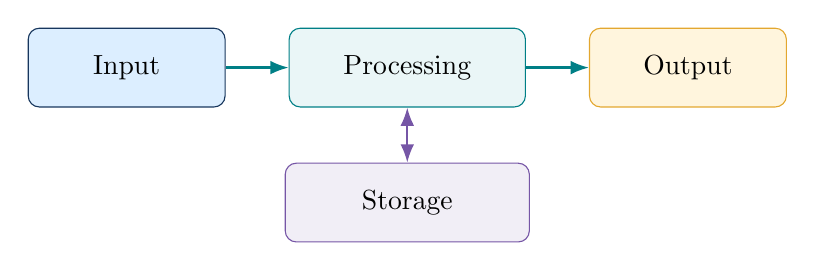
\begin{tikzpicture}[node distance=7mm and 8mm,>=Latex]
\node[draw=Navy,fill=Sky,rounded corners,minimum width=25mm,minimum height=10mm,align=center] (i) {Input};
\node[draw=Teal,fill=Pale,rounded corners,minimum width=30mm,minimum height=10mm,align=center,right=of i] (p) {Processing};
\node[draw=Gold,fill=LightGold,rounded corners,minimum width=25mm,minimum height=10mm,align=center,right=of p] (o) {Output};
\node[draw=Violet,fill=Violet!10,rounded corners,minimum width=31mm,minimum height=10mm,align=center,below=of p] (s) {Storage};
\draw[->,thick,Teal] (i)--(p);\draw[->,thick,Teal] (p)--(o);\draw[<->,thick,Violet] (p)--(s);
\end{tikzpicture}
\end{center}
\textit{Figure 1.2.} A simplified view of how computer components exchange information.

\section{CPU and its components}
The central processing unit (CPU) executes program instructions. The control unit coordinates operations, the arithmetic logic unit (ALU) performs arithmetic and logical comparisons, and registers hold small amounts of data immediately needed by the processor. Modern CPUs may contain multiple cores, allowing them to work on more than one stream of instructions.

\section{Memory and storage}
Primary memory includes RAM and ROM. RAM is volatile: its contents are normally lost when power is removed. ROM and other non-volatile memory retain information without continuous power. Cache is small, fast memory used to reduce the time needed to access frequently used data. Secondary storage, such as solid-state drives, hard disk drives, USB flash drives and memory cards, retains files and programs for longer periods.

\begin{center}
\begin{tabularx}{\textwidth}{p{.20\textwidth}XX}
\toprule
\textbf{Component} & \textbf{Main purpose} & \textbf{Important property}\\\midrule
RAM & Holds active programs and working data & Fast, volatile memory\\
ROM / firmware memory & Stores startup or device instructions & Non-volatile\\
Cache & Keeps frequently needed data close to CPU & Very fast, limited capacity\\
SSD / HDD & Stores files, applications and operating system & Non-volatile, larger capacity\\
\bottomrule
\end{tabularx}
\end{center}

\section{Input, output and peripheral devices}
Input devices include keyboards, mice, touchscreens, scanners, microphones, webcams, barcode readers, OCR and OMR equipment. Output devices include monitors, printers, speakers and projectors. A touchscreen can act as both input and output. Peripheral devices connect to a computer through interfaces such as USB, Bluetooth, HDMI or network connections.

\section{Choosing hardware for development}
Software development workloads vary. A basic editor and small Python scripts need modest resources, while virtual machines, large projects and data processing may require more memory, storage and CPU capacity. A developer should check operating-system support, available ports, upgrade options, reliability and backup requirements instead of choosing hardware by one specification alone.

\reviewtitle
\begin{enumerate}
\item Explain the input-processing-output cycle with one everyday example.
\item Distinguish the control unit and the arithmetic logic unit.
\item Compare RAM, ROM and cache memory.
\item Give four examples each of input and output devices.
\item What factors should a learner consider when selecting a computer for programming?
\end{enumerate}

\chapter{Data Representation in Computers}
Computers represent data using binary digits, 0 and 1. Electronic circuits can use two distinguishable states to encode these digits. Text, numbers, pictures, sound and video are all represented through patterns of bits, although the encoding rules differ.

\section{Bits, bytes and number systems}
A bit is a binary digit. A group of eight bits is called a byte. Larger quantities are commonly expressed using kilobytes, megabytes, gigabytes and terabytes; exact conventions may vary between decimal storage units and binary units such as KiB and MiB. Binary uses base 2, decimal uses base 10, octal uses base 8 and hexadecimal uses base 16.

\begin{center}
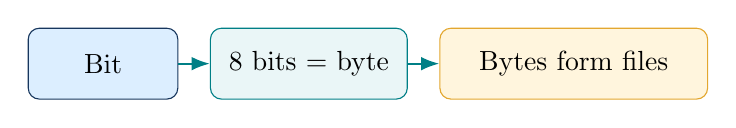
\begin{tikzpicture}[node distance=4mm,>=Latex]
\node[draw=Navy,fill=Sky,rounded corners,minimum width=19mm,minimum height=9mm] (b) {Bit};
\node[draw=Teal,fill=Pale,rounded corners,minimum width=25mm,minimum height=9mm,right=of b] (by) {8 bits = byte};
\node[draw=Gold,fill=LightGold,rounded corners,minimum width=34mm,minimum height=9mm,right=of by] (f) {Bytes form files};
\draw[->,thick,Teal] (b)--(by);\draw[->,thick,Teal] (by)--(f);
\end{tikzpicture}
\end{center}

\section{Converting number systems}
To convert a positive decimal integer to binary, repeatedly divide by two and record the remainders. Read the remainders from bottom to top. For example, decimal 13 becomes binary 1101 because \(13=8+4+1\). To convert binary 1011 to decimal, calculate \(1(2^3)+0(2^2)+1(2^1)+1(2^0)=11\).

Hexadecimal uses the symbols 0–9 and A–F, where A represents ten and F represents fifteen. One hexadecimal digit corresponds to four binary bits, making hexadecimal a compact way to read long binary values.

\section{Text, images and sound}
Character encodings assign numeric codes to characters. ASCII represents a basic set of characters; Unicode supports characters from many writing systems. UTF-8 is a widely used Unicode encoding for text on the web. Digital images use pixels and colour values; audio can be represented by samples taken at intervals. Image resolution, colour depth, sample rate and compression affect file size and quality.

\section{Data quality and safe handling}
Encoding does not guarantee that data is accurate. Developers must also validate inputs, use suitable data types, handle missing values and protect personal information. Files should have meaningful names and be backed up according to their importance.

\reviewtitle
\begin{enumerate}
\item Define bit and byte.
\item Convert decimal 13 to binary and show the method.
\item Convert binary 1011 to decimal.
\item Why is hexadecimal useful when working with binary values?
\item Distinguish ASCII and Unicode.
\end{enumerate}

\chapter{Basic Mathematics and Statistics for Computing}
Mathematics helps programmers describe relationships, compare values and reason about the behaviour of algorithms. Discrete mathematics focuses on distinct objects and structures, such as sets, logical statements, relations, functions, graphs and counting problems.

\section{Sets and operations}
A set is a collection of distinct elements. If \(A=\{1,2,3\}\) and \(B=\{3,4,5\}\), the union contains elements in either set, \(A\cup B=\{1,2,3,4,5\}\), while the intersection contains elements shared by both, \(A\cap B=\{3\}\). The difference \(A-B\) contains elements in A that are not in B. These ideas help model categories, permissions and relationships between data groups.

\section{Logic and truth values}
A proposition is a statement that can be true or false. Logical operators include AND, OR and NOT. In programming, conditions combine comparisons to decide which instructions should run. A truth table lists the possible inputs and resulting truth values and is useful when a condition becomes complicated.

\section{Relations, functions and graphs}
A relation describes a connection between elements. A function maps each valid input to exactly one output. Graphs consist of vertices and edges and can represent routes, social connections, network links or dependencies between tasks. Directed edges indicate direction; undirected edges represent a two-way relationship unless otherwise specified.

\section{Basic statistics}
Mean is the arithmetic average, median is the middle value after sorting, and mode is the most frequent value. Range is the difference between the maximum and minimum. Statistics help summarise test results, response times and software usage, but conclusions should consider sample size, data quality and unusual values.

\reviewtitle
\begin{enumerate}
\item Find the union and intersection of \(A=\{1,2,3\}\) and \(B=\{3,4,5\}\).
\item Explain AND, OR and NOT with simple examples.
\item Distinguish a relation from a function.
\item What are vertices and edges in a graph?
\item Find the mean and median of 4, 6, 7, 7 and 11.
\end{enumerate}

\chapter{Problem-Solving Methods}
Programming begins with understanding a problem, not with typing code. A reliable solution identifies the expected result, the available input, the rules that transform input into output and the special cases that may cause failure.

\photo{programming-code.png}{Writing and reviewing program code}{Figure 4.1. A programming editor helps developers write and inspect instructions; screenshot: Zhanjack822, Wikimedia Commons, CC0 1.0.}
\section{Define and analyse the problem}
Read the requirement carefully. Separate known facts from assumptions, identify constraints and ask questions where the requirement is unclear. Determine valid input ranges, expected output format and what should happen when data is missing or invalid. A small example often exposes misunderstandings early.

\section{Algorithms and pseudocode}
An algorithm is a finite, ordered set of steps for solving a problem. Good algorithms are clear, terminate, accept appropriate input and produce the required output. Pseudocode describes logic using plain structured language without committing to a particular programming language.

\begin{lstlisting}[style=webcode,language=Pseudo]
START
  INPUT first_number, second_number
  total = first_number + second_number
  OUTPUT total
STOP
\end{lstlisting}

\section{Flowcharts}
Flowcharts use standard symbols to show the flow of a process. An oval commonly represents start or end, a parallelogram represents input or output, a rectangle represents a process, and a diamond represents a decision. Arrows show the direction of control. A flowchart should be readable and avoid crossing lines where possible.

\section{Testing and debugging}
A test checks whether a program behaves as expected for selected input. Test normal values, boundary values, invalid input and empty input where relevant. A syntax error breaks the language rules; a runtime error occurs while the program runs; a logic error produces an incorrect result without necessarily crashing. Debugging means locating and correcting the cause, then rerunning tests.

\section{Efficiency and documentation}
Efficiency can involve execution time and memory use. For small problems, clarity is often the most important goal; for large inputs, algorithm choice can make a substantial difference. Comments should explain intent or non-obvious decisions, while documentation describes how to install, run and use the software.

\reviewtitle
\begin{enumerate}
\item List the main stages of problem solving.
\item Define an algorithm and state two qualities of a good algorithm.
\item Name four common flowchart symbols and their meanings.
\item Distinguish syntax, runtime and logic errors.
\item Why should a program be tested with boundary and invalid values?
\end{enumerate}

\chapter{Programming Language Concepts}
A programming language provides rules for expressing instructions that a computer can execute directly or through translation. Languages differ in syntax, type systems, abstraction, libraries, runtime environments and the kinds of problems for which they are commonly used.

\section{Machine, assembly and high-level languages}
Machine language consists of instructions encoded for a processor. Assembly language uses symbolic names for low-level instructions and is translated by an assembler. High-level languages such as Python, Java and C++ provide abstractions that make many programs easier to read and maintain.

\section{Compiler, interpreter and runtime}
A compiler translates source code into another form before execution; an interpreter executes instructions through a runtime process. Real language implementations may combine compilation, interpretation and virtual machines. A runtime provides services needed while a program executes, such as memory management or standard libraries.

\section{Syntax, semantics and paradigms}
Syntax describes the structure of valid expressions and statements. Semantics concerns their meaning. Procedural programming organises work into procedures or functions; object-oriented programming models data and behaviour through objects and classes; functional programming emphasises functions and expressions. Many languages support more than one paradigm.

\section{Development tools}
A code editor helps create and edit source files. An integrated development environment (IDE) may combine an editor, debugger, build tools, project navigation and testing support. Version control records changes over time and helps teams collaborate. Good naming, small functions, consistent formatting and clear commit messages improve maintainability.

\reviewtitle
\begin{enumerate}
\item Compare machine language, assembly language and high-level language.
\item Explain one difference between a compiler and an interpreter.
\item Distinguish syntax from semantics.
\item Describe procedural and object-oriented programming.
\item What features might an IDE provide?
\end{enumerate}

\chapter{Operating System Fundamentals}
An operating system (OS) manages the hardware resources of a computing device and provides services to applications. It offers a consistent way to work with files, memory, devices, processes and users. Examples include Windows, Linux, macOS, Android and iOS.

\photo{ubuntu-desktop.png}{Linux desktop environment}{Figure 6.1. The operating system provides the desktop, application launcher and workspace; screenshot: Canonical Limited, Wikimedia Commons, GPL.}
\section{Core responsibilities}
The OS schedules CPU time, manages memory, organises files, controls device access, provides a user interface and enforces security boundaries. It also detects certain errors and supports logging, networking and system updates. The kernel is the central component that manages privileged operations; shells and graphical interfaces allow users to interact with system services.

\section{Processes and memory}
A program is stored instructions; a process is a running instance of a program. The OS allocates CPU time and memory, tracks process states and coordinates input/output. Multitasking allows several tasks to make progress over time. Virtual memory helps manage address spaces and may use storage to extend the available memory model, though it is slower than RAM.

\section{Files, folders and permissions}
Files store content and folders organise files into a hierarchy. File names, extensions and metadata help users identify content. Permissions determine who may read, modify or execute files. Keep project files organised, use clear names, back up important data and avoid granting broader permissions than needed.

\section{User interfaces and maintenance}
A command-line interface accepts typed commands; a graphical user interface uses visual elements such as windows, menus and icons. Updates repair defects and address security issues. Install software from trusted sources, use standard user accounts for everyday work and keep recovery information available.

\reviewtitle
\begin{enumerate}
\item Define an operating system and give four examples.
\item Explain the roles of kernel and shell.
\item Distinguish a program and a process.
\item What is virtual memory?
\item State five safe computer-maintenance practices.
\end{enumerate}

\chapter{Computer Networks}
A computer network connects devices so they can exchange information and share services. Networks support web browsing, messaging, file transfer, printing, online learning and distributed applications. A network may be small and local or connect devices across continents.

\photo{lan-topology.png}{Local-area network topology}{Figure 7.1. A local-area network connects end devices through outlets, switches and a router; diagram: Mattias.Campe, Wikimedia Commons, CC BY-SA 3.0.}
\section{Network types and topologies}
A personal area network (PAN) connects nearby personal devices. A local area network (LAN) covers a limited site such as a home, laboratory or office. A wide area network (WAN) connects larger geographic areas. Common topologies include star, bus, ring and mesh; each has different cost, resilience and troubleshooting characteristics.

\section{Network devices}
A network interface connects a device to a network. Switches forward frames within a local network, while routers forward packets between networks. Wireless access points connect Wi-Fi devices. Modems or other access equipment connect a local network to an internet service. The exact device combination depends on the provider and network design.

\section{Addresses and name resolution}
A MAC address identifies a network interface at the link layer. An IP address supports logical addressing and routing. DNS translates domain names such as example.com into records used to locate services. DHCP can automatically assign network configuration such as IP addresses, gateway and DNS servers.

\section{Client-server and peer-to-peer}
In a client-server model, clients request services from servers. A web browser requesting a page is a common example. In peer-to-peer systems, devices can share responsibilities more directly. Both models require appropriate authentication, access control and safe handling of data.

\reviewtitle
\begin{enumerate}
\item Compare LAN and WAN.
\item Explain the purpose of a switch and a router.
\item Distinguish MAC and IP addresses.
\item What does DNS do?
\item Compare client-server and peer-to-peer models.
\end{enumerate}

\chapter{Transmission Media and Network Protocols}
Data travels through wired or wireless media. The medium affects speed, range, interference, installation cost and security. Network protocols define how devices format, address, transmit and interpret messages so that different systems can communicate.

\section{Guided and unguided media}
Twisted-pair copper cable is common in Ethernet LANs. Coaxial cable is used in some broadband and video systems. Optical fibre carries light and supports high bandwidth over long distances with low electromagnetic interference. Wireless communication uses radio waves, including Wi-Fi and cellular networks, and may be affected by walls, distance and interference.

\section{Protocol layers}
Layered networking divides a complex communication task into manageable responsibilities. Ethernet and Wi-Fi operate at the link level; IP provides addressing and routing; TCP offers reliable ordered delivery; UDP offers a simpler datagram service; HTTP and HTTPS support web communication. TLS helps protect communication against eavesdropping and tampering when configured correctly.

\section{Packets and ports}
Applications send data through protocols that may divide it into packets or segments. Port numbers help the operating system deliver traffic to the appropriate service. Firewalls can allow or block traffic according to rules. Open only the ports required for a service and keep network software updated.

\section{Troubleshooting connectivity}
Check power and physical connections first. Confirm Wi-Fi or Ethernet status, then inspect IP configuration and DNS resolution. Try to isolate whether the problem affects one device, one service or the whole network. Record error messages and change one variable at a time so the cause can be identified.

\reviewtitle
\begin{enumerate}
\item Compare twisted-pair cable and optical fibre.
\item Explain why network protocols are needed.
\item Distinguish TCP and UDP at a high level.
\item What is the role of a port number?
\item List a sensible sequence for troubleshooting a network connection.
\end{enumerate}

\chapter{Network Security}
Network security protects systems, communications and information from unauthorised access, misuse and disruption. Security depends on technology and human behaviour: even well-designed systems can be exposed by weak passwords, unpatched software, unsafe configuration or deceptive messages.

\photo{router-vlan.png}{Router and virtual LANs}{Figure 9.1. A router can route traffic between separate virtual LANs; diagram: Anatoly099, Wikimedia Commons, CC BY-SA 4.0.}
\section{Threats and vulnerabilities}
Malware includes viruses, worms, trojans, ransomware and spyware. Phishing attempts to trick people into revealing information or running unsafe files. Password attacks, unpatched services, misconfiguration and denial-of-service attacks can affect confidentiality, integrity or availability. A vulnerability is a weakness that a threat may exploit.

\section{Security controls}
Use strong unique passwords and multifactor authentication where available. Apply updates, use endpoint protection, enable firewalls and restrict privileges. Back up important information and test restoration. Encrypt sensitive data in transit and at rest where appropriate. Security controls should be selected based on the risks and the value of the information being protected.

\section{Safe network behaviour}
Verify unexpected links and attachments through a trusted channel. Avoid entering credentials on unfamiliar pages. Use secure Wi-Fi configurations and be cautious on public networks. Do not share passwords or one-time codes. Report suspicious activity promptly and preserve relevant details according to organisational procedure.

\section{Incident response}
A basic response includes identifying the event, limiting further harm, informing the appropriate people, preserving evidence, recovering safely and reviewing what can be improved. Do not attempt to hide an incident or destroy records. Follow organisational policy and applicable law.

\reviewtitle
\begin{enumerate}
\item Define malware, phishing and vulnerability.
\item Explain the confidentiality, integrity and availability goals of security.
\item Give five ways to protect a computer on a network.
\item Why are backups and restoration tests important?
\item List the main stages of a basic incident response.
\end{enumerate}

\chapter{Python Basics}
Python is a high-level, general-purpose programming language used for automation, data analysis, web development, scientific computing and many other tasks. Its readable syntax makes it suitable for learning programming concepts while still supporting large applications.

\photo{python-simulation.jpg}{Python programming}{Figure 10.1. A Python program can combine source code and a visual output window; screenshot: MikeRun, Wikimedia Commons, CC BY-SA 4.0.}
\section{Installing and running Python}
Use the official Python distribution or an approved environment. The interpreter executes Python statements. IDLE is a simple environment that includes an editor and interactive shell; other editors and IDEs are also available. Check the installation by running a short command and confirming the version reported by the system.

\begin{lstlisting}[style=webcode,language=Python]
print("Hello, learner!")
name = input("Enter your name: ")
print("Welcome,", name)
\end{lstlisting}
The first line displays a message. The second reads text from the user and stores it in a variable. The final line combines output with the entered value.

\section{Variables, names and data types}
A variable is a name that refers to a value. Identifiers should be meaningful and follow Python's naming rules. Common types include int for integers, float for floating-point numbers, str for text, bool for true/false values, and collections such as list, tuple, set and dict. Python is case-sensitive, so \texttt{score} and \texttt{Score} are different names.

\section{Operators and expressions}
Arithmetic operators include +, -, *, /, //, \% and **. Comparison operators include ==, !=, <, >, <= and >=. Logical operators and, or and not combine conditions. Parentheses make complicated expressions easier to read. Use explicit conversion such as \texttt{int(input(...))} when numeric input is required, and handle invalid input where necessary.

\section{Comments, indentation and errors}
Comments begin with the hash symbol. Indentation defines blocks in Python and must be consistent. Syntax errors prevent code from being parsed; exceptions occur during execution; logic errors produce the wrong answer. Read tracebacks from the final error message and inspect the relevant line before changing code.

\reviewtitle
\begin{enumerate}
\item State four common uses of Python.
\item Write a program that displays a message and reads a user's name.
\item Compare int, float, str and bool.
\item Explain the difference between \texttt{=} and \texttt{==}.
\item Why is indentation important in Python?
\end{enumerate}

\chapter{Control Structures}
Control structures determine the order in which instructions run. Sequence executes statements in order, selection chooses between alternatives, and iteration repeats a block. These structures allow a program to respond to input and process collections of data.

\section{Selection with if}
An \texttt{if} statement runs a block when a condition is true. \texttt{elif} checks another condition, and \texttt{else} provides a fallback. Conditions may use comparison and logical operators.

\begin{lstlisting}[style=webcode,language=Python]
marks = int(input("Enter marks: "))
if marks >= 80:
    print("Grade A")
elif marks >= 60:
    print("Grade B")
elif marks >= 40:
    print("Grade C")
else:
    print("Needs improvement")
\end{lstlisting}
The order matters: the most restrictive threshold is tested first. Validate input ranges if marks must lie between 0 and 100.

\section{Iteration with for and while}
A \texttt{for} loop is useful for iterating over a sequence or range. A \texttt{while} loop repeats while a condition remains true. Each loop should make progress toward termination unless it is intentionally designed to run continuously.

\begin{lstlisting}[style=webcode,language=Python]
for number in range(1, 6):
    print(number)

count = 3
while count > 0:
    print(count)
    count -= 1
\end{lstlisting}

\section{Loop control and tracing}
\texttt{break} exits a loop and \texttt{continue} skips to the next iteration. A trace table records variable values at each step and is useful for checking a loop's logic. Avoid changing many variables in a single step when debugging a beginner program.

\reviewtitle
\begin{enumerate}
\item Compare sequence, selection and iteration.
\item Write an if-else program to determine whether a number is even or odd.
\item What is the difference between for and while loops?
\item Explain break and continue.
\item Trace a loop that prints numbers from 1 to 5.
\end{enumerate}

\chapter{Functions}
A function is a named block of code that performs a defined task. Functions help divide a problem into smaller parts, avoid repeated code and make programs easier to test. A function can receive inputs called parameters and return a result.

\section{Defining and calling functions}
Use the \texttt{def} keyword to define a function. The indented body contains the instructions. Calling a function runs that body; a return statement sends a value back to the caller.

\begin{lstlisting}[style=webcode,language=Python]
def rectangle_area(length, width):
    return length * width

area = rectangle_area(8, 3)
print("Area:", area)
\end{lstlisting}

\section{Parameters, arguments and scope}
Parameters appear in the function definition; arguments are values supplied when it is called. Local variables are created within a function and normally cannot be accessed directly outside it. Default parameters can make an argument optional. Choose names that communicate the purpose of each value.

\section{Built-in and user-defined functions}
Python provides built-in functions such as \texttt{print}, \texttt{input}, \texttt{len}, \texttt{type}, \texttt{sum}, \texttt{min} and \texttt{max}. User-defined functions capture a task specific to a program. A useful function has a clear responsibility, predictable inputs and outputs, and a name that explains its role.

\section{Testing functions}
Test normal cases, boundary values and invalid inputs. A function that calculates a percentage should define what happens when the total is zero. Small tests make errors easier to isolate and allow later changes without manually checking every part of the application.

\reviewtitle
\begin{enumerate}
\item Define a function and state two benefits.
\item Write a function that returns the square of a number.
\item Distinguish parameters and arguments.
\item What is the purpose of return?
\item Why should functions be tested with boundary values?
\end{enumerate}

\chapter{Strings}
A string is an immutable sequence of characters. Strings represent names, messages, addresses, codes and other text. Because strings are immutable, an operation that appears to change a string normally returns a new string rather than altering the original object.

\section{Creating and accessing strings}
Strings can be written with single or double quotes. Triple quotes can represent multiline text. Indexing accesses a character; positive indexes start at zero, while negative indexes count from the end. Slicing selects a range and uses an exclusive stop index.

\begin{lstlisting}[style=webcode,language=Python]
word = "Python"
print(word[0])      # P
print(word[-1])     # n
print(word[1:4])    # yth
print(len(word))    # 6
\end{lstlisting}

\section{String methods}
Useful methods include \texttt{lower}, \texttt{upper}, \texttt{strip}, \texttt{replace}, \texttt{split}, \texttt{join}, \texttt{startswith} and \texttt{endswith}. The \texttt{in} operator checks whether a substring is present. Methods should be selected based on the intended transformation and the format of the input.

\section{Formatting and validation}
F-strings make it convenient to insert values into text, for example \texttt{f"Hello, \{name\}"}. User input should be validated for expected length, allowed characters and required format. Validation is not the same as security by itself; applications should also apply context-appropriate encoding and access controls.

\reviewtitle
\begin{enumerate}
\item What does it mean that strings are immutable?
\item Explain indexing and slicing.
\item Name five useful string methods.
\item Write code to convert a name to uppercase and remove surrounding spaces.
\item Why should user-provided text be validated?
\end{enumerate}

\chapter{Lists}
A list is an ordered, mutable collection that can hold multiple values. Lists are useful when a program needs to store, examine, sort or update a group of items. List elements can have different types, although collections with a consistent type are often easier to work with.

\section{Creating and accessing lists}
A list uses square brackets. Indexing retrieves an element and slicing retrieves a sublist. Lists support updates, append, insert, remove, pop, sort and reverse. These operations change the list in different ways, so consult the method's purpose before using it.

\begin{lstlisting}[style=webcode,language=Python]
scores = [72, 85, 64, 91]
scores.append(78)
scores[0] = 75
print(scores)
print("Count:", len(scores))
print("Highest:", max(scores))
\end{lstlisting}

\section{Traversing and processing}
A for loop can visit each element. A running total can calculate a sum, and a condition can count values that meet a requirement. Python also provides built-in functions and comprehensions for common transformations. Begin with a clear loop when learning, then use concise expressions when their meaning remains easy to understand.

\section{Nested lists and common mistakes}
A list can contain other lists, which can represent rows and columns. Indexing outside the valid range raises an error. Removing an item while iterating over the same list can lead to skipped values; when filtering, creating a new list is often safer.

\reviewtitle
\begin{enumerate}
\item Define a list and explain why it is mutable.
\item Write a program to find the sum of numbers in a list.
\item Compare append, insert and remove.
\item What is a nested list?
\item Describe two common list errors and how to avoid them.
\end{enumerate}

\chapter{Tuples and Dictionaries}
Tuples and dictionaries organise related data in different ways. A tuple is ordered and immutable. A dictionary maps unique keys to values and is useful when values need to be retrieved by a meaningful label.

\section{Tuples}
Tuples are written using commas, often inside parentheses. They are useful for fixed groups of values, such as coordinates or a returned pair of results. A one-element tuple requires a trailing comma. Since tuples are immutable, their element assignments cannot be changed after creation.

\section{Dictionaries}
A dictionary uses key-value pairs. Keys must be hashable and unique within the dictionary. Values can be updated, added or removed. Methods such as \texttt{keys}, \texttt{values}, \texttt{items}, \texttt{get}, \texttt{update} and \texttt{pop} support common operations.

\begin{lstlisting}[style=webcode,language=Python]
learner = {
    "name": "Ananya",
    "grade": 11,
    "active": True
}
print(learner["name"])
learner["grade"] = 12
print(learner.get("course", "Not assigned"))
\end{lstlisting}

\section{Choosing a collection}
Use a list when order and changeable elements are important. Use a tuple for a fixed sequence. Use a dictionary when a key should identify a value. Choose the structure that makes the data and intended operations easiest to understand.

\reviewtitle
\begin{enumerate}
\item Compare lists and tuples.
\item Why must dictionary keys be unique?
\item Write a dictionary describing a book with three fields.
\item Explain the difference between dictionary indexing and get.
\item Give one suitable use for each of list, tuple and dictionary.
\end{enumerate}

\chapter{Introduction to Data Structures}
A data structure is a way of organising data so that operations can be performed effectively. Different structures support different patterns of access, insertion, deletion and searching. Choosing a suitable structure can improve clarity and performance.

\section{Abstract data types and operations}
An abstract data type describes the behaviour expected from a collection without requiring one specific implementation. Common operations include insert, delete, search, traverse and update. A stack, for example, supports adding and removing items at one end; a queue processes items in arrival order.

\section{Linear and non-linear structures}
Linear structures arrange elements in a sequence, as in arrays, linked lists, stacks and queues. Non-linear structures express branching or network relationships, as in trees and graphs. A structure's usefulness depends on the problem rather than on whether it is more advanced.

\photo{stack-queue.png}{Stack and queue comparison}{Figure 14.1. A stack follows last-in, first-out order, while a queue follows first-in, first-out order; diagram: Choteseeworld, Wikimedia Commons, CC BY-SA 4.0.}

\section{Selecting a structure}
Consider the data's relationships, the operations used most often, memory constraints and implementation complexity. For frequent lookup by key, a dictionary or hash table may be appropriate. For hierarchical information, a tree may fit naturally. For ordered processing, a queue may be the simplest model.

\reviewtitle
\begin{enumerate}
\item Define a data structure.
\item List five common data-structure operations.
\item Compare linear and non-linear structures.
\item Give one real-world example of a stack and a queue.
\item What factors influence the choice of a data structure?
\end{enumerate}

\chapter{Linear Data Structures}
Linear data structures arrange elements in a sequence. Arrays, linked lists, stacks and queues are common examples. Each offers a different balance between access speed, insertion, deletion and memory organisation.

\section{Arrays}
An array stores elements in indexed positions. Index-based access is efficient when the position is known. Inserting or deleting elements in the middle may require moving other values. Python lists behave like dynamic arrays for many common uses.

\section{Linked lists}
A linked list contains nodes. Each node stores data and one or more links to other nodes. A singly linked list points to the next node; a doubly linked list points both forward and backward. Linked lists can insert or remove nodes efficiently when the relevant position is known, but finding a distant element usually requires traversal from the start.

\section{Stacks}
A stack follows last-in, first-out (LIFO). The main operations are push, pop and peek. A stack models undo operations, function calls and expression evaluation. Removing from an empty stack should be handled as an error or an explicitly defined empty result.

\section{Queues}
A queue follows first-in, first-out (FIFO). Enqueue adds an item and dequeue removes the oldest item. Queues model print jobs, service requests and tasks waiting for processing. Circular queues can reuse array space, while priority queues process items according to priority rather than arrival order.

\begin{center}
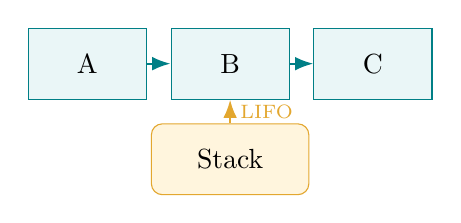
\begin{tikzpicture}[node distance=3mm,>=Latex]
\node[draw=Teal,fill=Pale,minimum width=15mm,minimum height=9mm] (a) {A};
\node[draw=Teal,fill=Pale,minimum width=15mm,minimum height=9mm,right=of a] (b) {B};
\node[draw=Teal,fill=Pale,minimum width=15mm,minimum height=9mm,right=of b] (c) {C};
\node[draw=Gold,fill=LightGold,rounded corners,minimum width=20mm,minimum height=9mm,below=of b] (s) {Stack};
\draw[->,thick,Teal] (a)--(b);\draw[->,thick,Teal] (b)--(c);
\draw[->,thick,Gold] (s)--node[right,font=\scriptsize]{LIFO} (b);
\end{tikzpicture}
\end{center}
\textit{Figure 15.1.} Sequence-based structures support different ways of adding and removing items.

\reviewtitle
\begin{enumerate}
\item Compare arrays and linked lists.
\item Explain the LIFO rule with an example.
\item Explain the FIFO rule with an example.
\item What do push, pop, enqueue and dequeue mean?
\item Which structure would you consider for a printer queue, and why?
\end{enumerate}

\chapter{Non-Linear Data Structures}
Non-linear data structures represent branching or many-to-many relationships. Trees are hierarchical; graphs model general connections. These structures appear in file systems, routing, dependency analysis, maps and social networks.

\section{Trees and terminology}
A tree consists of nodes connected by edges and has a root node. A parent can have child nodes; a node without children is a leaf. A subtree is a node together with its descendants. A binary tree allows each node to have at most two children. A binary search tree arranges values so that values in the left subtree are smaller and values in the right subtree are larger, according to its ordering rule.

\section{Tree traversal}
Pre-order visits root, left subtree, right subtree. In-order visits left subtree, root, right subtree. Post-order visits left subtree, right subtree, root. For a binary search tree, in-order traversal visits keys in sorted order if the tree follows the required ordering rules.

\section{Graphs}
A graph consists of vertices and edges. It can be directed or undirected, weighted or unweighted. A path is a sequence of connected vertices; a cycle returns to a previously visited vertex. Graphs can be represented by an adjacency list or adjacency matrix. An adjacency list stores neighbours for each vertex, while a matrix records whether pairs of vertices are connected.

\section{Applications}
Trees can represent folders, organisational structures and syntax. Graphs can represent road networks, computer networks and links between web pages. The representation should match the expected operations and the size and density of the structure.

\reviewtitle
\begin{enumerate}
\item Define root, parent, child and leaf in a tree.
\item Explain pre-order, in-order and post-order traversal.
\item What is a binary search tree?
\item Compare directed and undirected graphs.
\item Compare adjacency lists and adjacency matrices.
\end{enumerate}

\chapter{Integrated Practice and Revision}
\section{Scenario: a learner-results application}
A school wants a small program that stores learner names and marks, calculates class summaries and produces a report. Begin by clarifying the expected input, valid mark range and output format. Select suitable data structures, write an algorithm, implement the solution in Python and test it with normal, boundary and invalid values.

\section{Suggested design}
Use a list to hold marks and a dictionary when each learner needs a labelled record. Create small functions to validate marks, calculate summaries and format output. Handle an empty list before calculating an average. Keep the program's responsibilities separate so that changes to input or output do not require rewriting the calculation logic.

\begin{lstlisting}[style=webcode,language=Python]
def average(values):
    if not values:
        return None
    return sum(values) / len(values)

marks = [72, 85, 64, 91]
result = average(marks)
if result is None:
    print("No marks available")
else:
    print(f"Average: {result:.2f}")
\end{lstlisting}

\section{Testing plan}
Test an ordinary list of marks, a list containing one value, an empty list, values at the allowed boundaries and invalid values. Check whether the program returns a sensible result, communicates errors clearly and avoids dividing by zero. Record defects and rerun the tests after making changes.

\section{Final revision questions}
\begin{enumerate}
\item Describe the main functional units of a computer system.
\item Explain how binary represents data and convert a simple decimal integer to binary.
\item Explain sets, logical operators and functions with examples.
\item Describe the stages of problem analysis, algorithm design, implementation and testing.
\item Compare high-level languages, compilers and interpreters.
\item Explain the responsibilities of an operating system.
\item Compare LAN and WAN and describe the roles of switches and routers.
\item Explain the purpose of IP, TCP, DNS and HTTPS.
\item List practical measures for protecting a computer and network.
\item Write a Python program using selection to classify a number as positive, negative or zero.
\item Write a loop that calculates the total of a list of numbers.
\item Define a function that returns the largest of three values.
\item Explain string indexing and slicing.
\item Compare list, tuple and dictionary with examples.
\item Compare stack and queue and identify their processing order.
\item Explain the difference between a tree and a graph.
\end{enumerate}

\section{Study and problem-solving approach}
For a definition question, provide a clear meaning and one example. For a comparison, state the distinguishing feature and explain where each option is useful. For a programming question, identify the input, outline the logic, write readable code and describe the expected output. Test assumptions rather than relying on a single example. When code fails, read the error message, isolate the smallest failing case and change one thing at a time.

\end{document}
